\documentclass{article}
\usepackage[utf8]{inputenc}
\usepackage{graphicx}

\title{Homework 8 Text Answers}
\author{Matthew Wong}
\date{March 3, 2022}

\begin{document}
\maketitle

\begin{enumerate}
\setcounter{enumi}{2}
\item
  \begin{enumerate}
  \item
    After the \texttt{ls} command finishes running, the Python shell is exited. This is because the
    \texttt{exec} command replaces the current process with another process, so the original Python
    process is terminated.
  \end{enumerate}

\setcounter{enumi}{4}
\item
  Coin toss simulation:
\begin{figure}[!hb]
  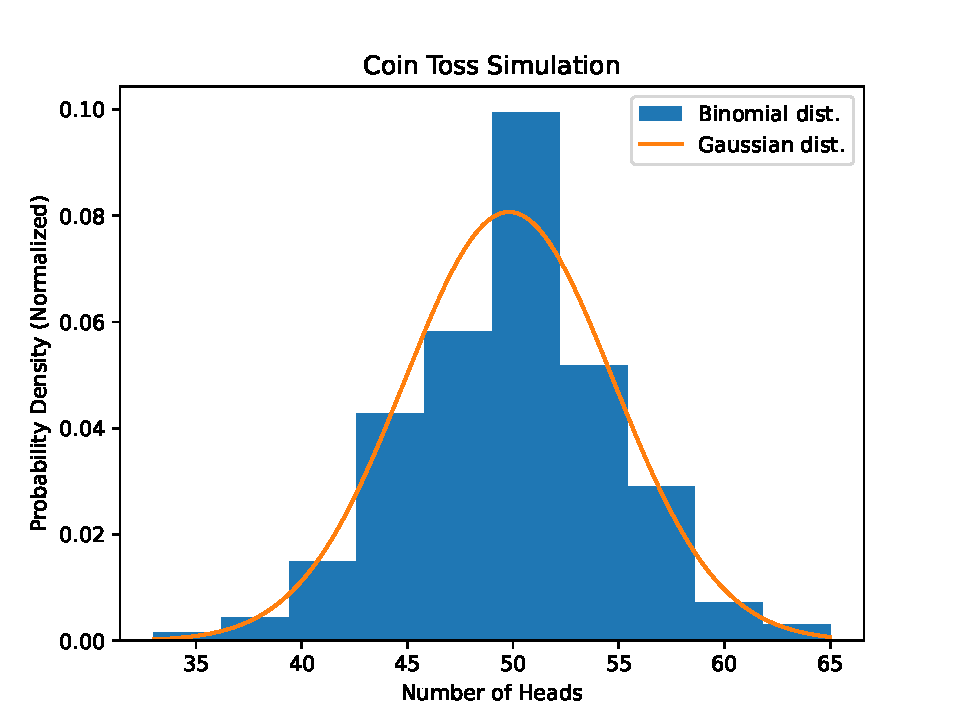
\includegraphics[width=\textwidth]{coinchart.pdf}
  \caption{A binomial distribution of a coin toss simulation with a Gaussian distribution
    overplotted}
  \centering
\end{figure}

\end{enumerate}
\end{document}
